
\subsection{模型检验}
最后,本文根据前四年的交易数据,基于以上方法制定了优化后的订购方案。
并通过计算机按照数据统计分布规律生成随机供货偏差取代优化模型中期望值的方式进行仿真模拟。
在仿真情况下,按照前文制定的方案进行订购和转运时,企业每周的订货量如下图所示:


\begin{center} {\centering
\vbox{
	\centerline{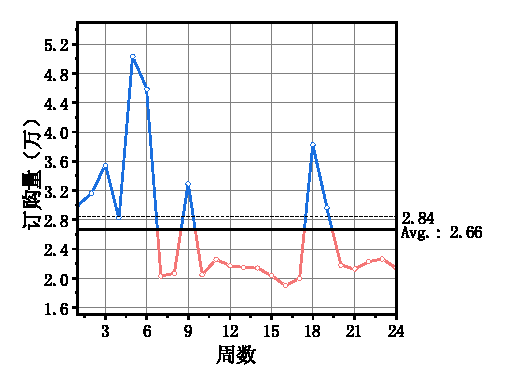
\includegraphics[width=8cm]{Image/final test.eps}}
	\vskip 1mm{\small
	图8\quad 企业总订货量变化.\label{lstm}
	\\}
	}
	}
\end{center}

由图可知,企业的订货量较平稳,且略高于满足两周生产需求的原材料数量,有效地节约了仓储成本、保证了生产进度。
由于后期供应商的总体供货疲软,在预测模型的指导下,企业在前期采取了一定的囤货行为,这虽然花费了较多的存储成本,但使总产量上升,总体有利。
本文认为,针对问题2制定的订购及转运方案实施效果良好,进一步提高了企业生产的经济效益。
